%%%%%%%%%%%%%%%%%%%%%%%%%%%%%%%%%%%%%%%%%
% Beamer Presentation
% LaTeX Template
% Version 1.0 (10/11/12)
%
% This template has been downloaded from:
% http://www.LaTeXTemplates.com
%
% License:
% CC BY-NC-SA 3.0 (http://creativecommons.org/licenses/by-nc-sa/3.0/)
%
%%%%%%%%%%%%%%%%%%%%%%%%%%%%%%%%%%%%%%%%%

%----------------------------------------------------------------------------------------
%	PACKAGES AND THEMES
%----------------------------------------------------------------------------------------

\documentclass{beamer}

\mode<presentation> {

% The Beamer class comes with a number of default slide themes
% which change the colors and layouts of slides. Below this is a list
% of all the themes, uncomment each in turn to see what they look like.

%\usetheme{default}
%\usetheme{AnnArbor}
%\usetheme{Antibes}
%\usetheme{Bergen}
%\usetheme{Berkeley}
%\usetheme{Berlin}
\usetheme{Boadilla}
%\usetheme{CambridgeUS}
%\usetheme{Copenhagen}
%\usetheme{Darmstadt}
%\usetheme{Dresden}
%\usetheme{Frankfurt}
%\usetheme{Goettingen}
%\usetheme{Hannover}
%\usetheme{Ilmenau}
%\usetheme{JuanLesPins}
%\usetheme{Luebeck}
%\usetheme{Madrid}
%\usetheme{Malmoe}
%\usetheme{Marburg}
%\usetheme{Montpellier}
%\usetheme{PaloAlto}
%\usetheme{Pittsburgh}
%\usetheme{Rochester}
%\usetheme{Singapore}
%\usetheme{Szeged}
%\usetheme{Warsaw}

% As well as themes, the Beamer class has a number of color themes
% for any slide theme. Uncomment each of these in turn to see how it
% changes the colors of your current slide theme.

%\usecolortheme{albatross}
%\usecolortheme{beaver}
%\usecolortheme{beetle}
%\usecolortheme{crane}
%\usecolortheme{dolphin}
\usecolortheme{dove}
%\usecolortheme{fly}
%\usecolortheme{lily}
%\usecolortheme{orchid}
%\usecolortheme{rose}
%\usecolortheme{seagull}
%\usecolortheme{seahorse}
%\usecolortheme{whale}
%\usecolortheme{wolverine}

%\setbeamertemplate{footline} % To remove the footer line in all slides uncomment this line
%\setbeamertemplate{footline}[page number] % To replace the footer line in all slides with a simple slide count uncomment this line

%\setbeamertemplate{navigation symbols}{} % To remove the navigation symbols from the bottom of all slides uncomment this line
}
\usepackage{graphicx} % Allows including images
\usepackage{booktabs} % Allows the use of \toprule, \midrule and \bottomrule in tables
\usepackage{ifthen}
\usepackage{uniprpres}
\usepackage{color}

%----------------------------------------------------------------------------------------
%	TITLE PAGE
%----------------------------------------------------------------------------------------



\titolo{Estrazione di punti operazione per AGV industriali da scansioni laser terrestri}
\titoloIng{Automatic extraction of AGV pickup and delivery points from terrestrial laser scan data}
\laureando{Giorgio Ghisotti}
\annoaccademico{2016-2017}
\corsodilaurea{Ingegneria Informatica, Elettronica e delle Telecomunicazioni}
\relatore[Chiar.mo Prof.]{Jacopo Aleotti}
\correlatorea[Ing.]{Mikhail Giorgini}

\begin{document}
\maketitle

\begin{frame}
	\frametitle{Il Problema}
	\vskip 0.4cm
	\begin{center}
		\begin{huge}
			Trovare automaticamente punti operazione per carrelli automatici (AGV)
		\end{huge}
	\end{center}
\vskip 0.4cm
\begin{center}
	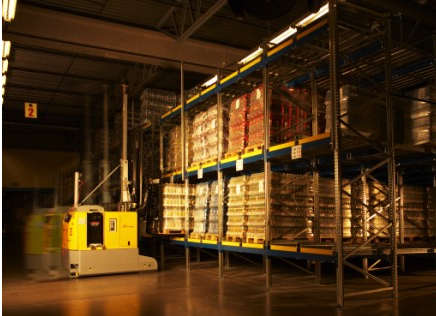
\includegraphics[scale=0.5]{Img/LGV/op}
\end{center}
\end{frame}
\begin{frame}
	\frametitle{Come si procedeva prima}
	\begin{columns}
		\column{0.6\textwidth}
			\begin{large}
				\begin{itemize}
					\item Misurazioni manuali sul campo
					\begin{itemize}
						\item Effettuate conducendo un carrello in giro per il magazzino
						\item Richiedevano mesi
						\item Rendevano inagibili parti del magazzino durante la procedura
					\end{itemize}
					\item Individuazione manuale con l'aiuto di un programma
					\begin{itemize}
						\item Procedura tediosa
						\item Richiede settimane
						\item Occupa l'operatore per molto tempo
					\end{itemize}
				\end{itemize}
			\end{large}
		\column{0.4\textwidth}
		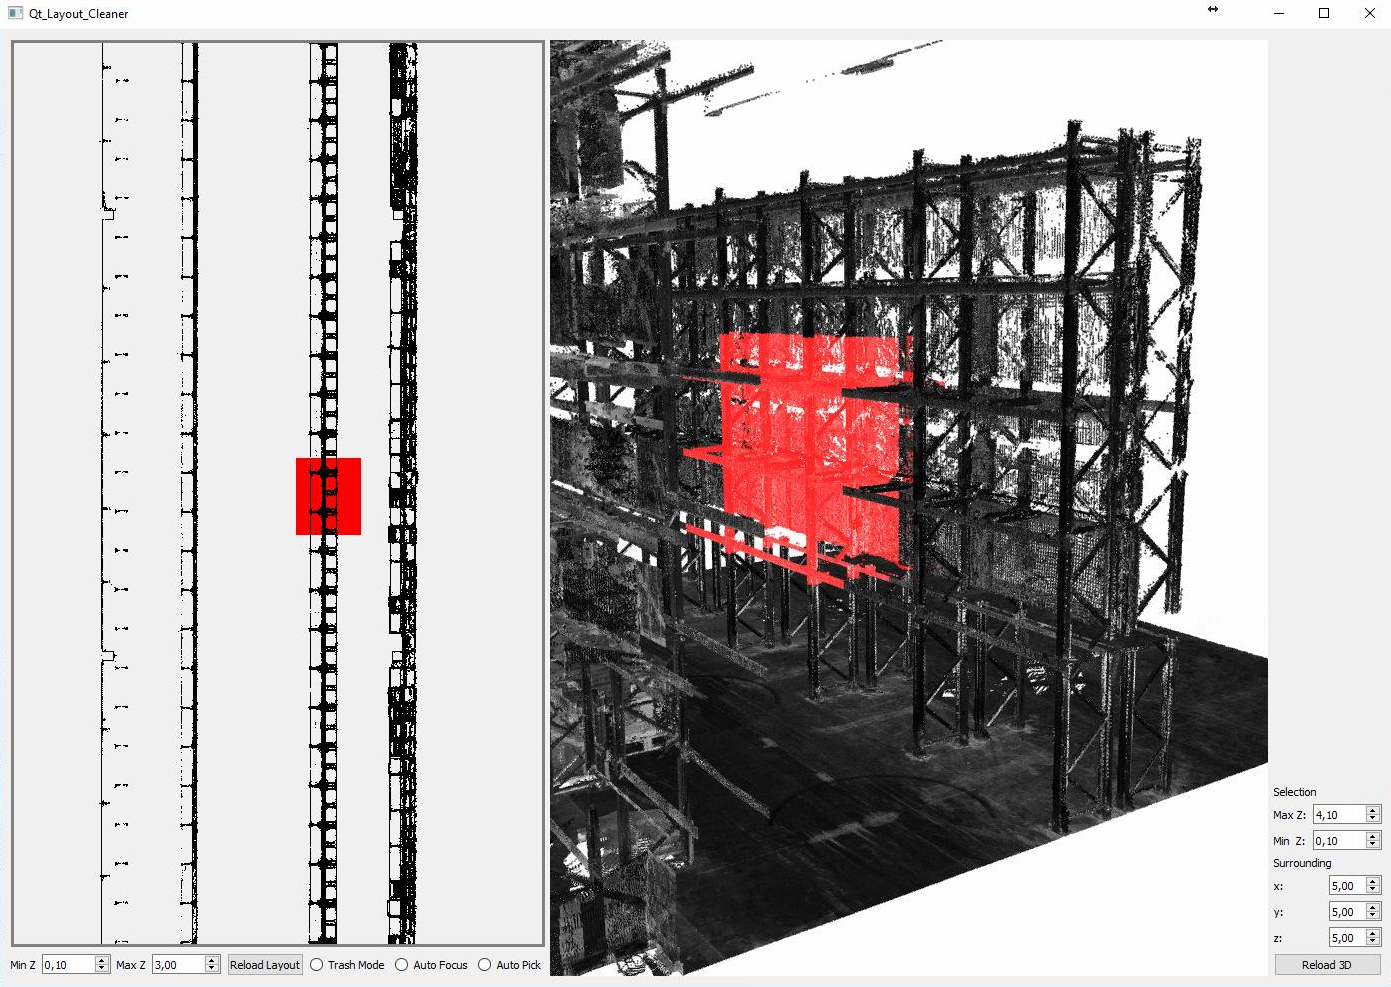
\includegraphics[width=\textwidth]{Img/LGV/select}
	\end{columns}
\end{frame}
\begin{frame}
	\frametitle{Dalla Point Cloud al 2D}
\end{frame}



























\end{document} 